\section{Related Work}
\paragraph{Spatial reasoning and constructive generation.}
Paper-folding and program-to-geometry benchmarks test how models derive geometric answers from visual or symbolic information~\cite{zhou2026paperfolding,luo2026geogrambench}. Brick assembly asks for an executable spatial output: a collection of discrete placements that can be checked for coverage, overlap, and connection. MeshGPT and LLaMA-Mesh represent 3D geometry as token sequences~\cite{meshgpt,llamamesh}. Our sequence encodes rectangular footprints and absolute grid positions.

\paragraph{Brick assembly and stability.}
Prior work treats brick assembly as graph generation, sequential construction, or structure understanding~\cite{thompson2020lego,brickbybrick,breakandmake}. BrickGPT uses autoregressive placement sequences and physics-aware rollback~\cite{brickgpt}. BrickNet represents a wider range of parts and connectors with an assembly graph~\cite{bricknet}. BrickForma imposes a single stud-connected component by reconstructing the predicted volume. Force-balance screening, as studied by StableLego~\cite{stablelego}, requires a separate mechanical model.

\paragraph{Procedural supervision.}
Procedural generation offers control over shape variation and scale~\cite{infinigen}. SpatialVLM uses synthetic supervision to teach spatial relations to a vision--language model~\cite{spatialvlm}. BrickForma uses a language model to author executable generators, checks their geometric outputs algorithmically, and trains a text-only model on the resulting text--placement pairs using LoRA~\cite{lora}.

\section{From Programs to Checked Training Data}
\label{sec:dataset}
\subsection{Parametric Programs and Shared Geometry}
GPT-6.1 Sol assists in writing parameterized programs for 21 object categories. Each program defines an object family through part dimensions, proportions, openings, and support arrangements. Executing the programs gives 80,000 source voxel models in two 40,000-model shards on a $48^3$ grid, with 750--1,250 occupied cells per object. Exact and canonical occupancy hashes over 48 axis/sign transforms found no cross-shard duplicates. Geometry plans and version identifiers accompany the records (Figure~\ref{fig:data-workflow}).

BrickMore-48 pairs each shape with five bilingual descriptions. L1 expresses the object and its main parts, while progressively richer descriptions add structure, proportions, appearance, and views. The geometry is shared by all five levels, so the same target provides supervision for both concise and detailed requests. Appendix~\ref{app:dataset} gives a birdhouse example.

\subsection{Voxel-to-Brick Conversion}
The conversion tiles each layer with same-color rectangular footprints and inspects the resulting stud components. Local bridging and retiling address ungrounded components, with edits recorded against the source voxels. The retile release raises the geometry-pass count from 65,503 to 79,298, recovering 13,795 failures. Across the corpus it adds 228,582 and removes 125 voxels, and 31,532 passing models require no edits.

The release checks that the target voxels are six-neighbor connected, every brick component is grounded, and brick placement exactly covers the derived target. Several individually grounded brick components may pass these release checks. Inference uses a stricter single-component constraint. Contact-based gravity screening records a separate outcome (Appendix~\ref{app:dataset}).

\subsection{Integrated Release and Training Corpus}
The full retile release contains 702 geometry failures. A revised batch-B piano release passes all 1,905 slots where the full retile release passed 1,902, giving a report-derived integrated count of $79{,}298-1{,}902+1{,}905=79{,}301$. Table~\ref{tab:training-data} reports the release and recorded fine-tuning counts.
\begin{table}[t]
\centering
\small
\setlength{\tabcolsep}{4pt}
\begin{tabular}{lr}
\toprule
\multicolumn{2}{l}{\emph{Dataset (release reports)}} \\
\midrule
Source models / categories / grid & 80,000 / 21 / $48^3$ \\
Bilingual caption records & 400,000 \\
Failing in full retile release & 702 (0.88\%) \\
Passing in full retile release & 79,298 \\
Piano models restored by revised release & 3 \\
Integrated passing models & 79,301 \\
\midrule
\multicolumn{2}{l}{\emph{Fine-tuning corpus}} \\
\midrule
(model, English caption) samples & 396,610 \\ % Training manifest confirmation pending
Training / validation samples & 356,955 / 39,655 \\
Tokens over 3 epochs & 2,228,044,818 \\ % Training manifest confirmation pending
\bottomrule
\end{tabular}
\caption{Dataset and fine-tuning corpus. The two blocks are counted separately: the upper block from the dataset release reports, the lower block as recorded for the fine-tuning run.}
\label{tab:training-data}
\end{table}

\begin{algorithm}[tb]
\caption{BrickForma inference and retiling}
\label{alg:inference-retiling}
\small
\begin{algorithmic}[1]
\REQUIRE prompt $c$; fine-tuned model $\theta$; library $\mathcal{L}$ (20 footprints); seeds $S=(42,104,2026)$; MILP tiers $T=(12,60,180)$\,s
\ENSURE $(B_{\mathrm{out}}, \textit{status})$, $\textit{status}\in\{\textsc{Success},\textsc{Draft},\textsc{Failed}\}$
\STATE $B \gets \emptyset$; $A \gets \emptyset$
\FOR{$s \in S$}
  \STATE $(B_s,\textit{rep}) \gets \mathrm{Parse}(\theta.\mathrm{Generate}(c,\ \mathrm{seed}{=}s))$
  \STATE $A \gets A \cup \{(B_s,\textit{rep})\}$
  \IF{$\textit{rep}.\mathrm{complete} \land \textit{rep}.\mathrm{valid}$}
    \STATE $B \gets B_s$; \textbf{break}
  \ENDIF
\ENDFOR
\IF{$B=\emptyset$}
  \IF{no completed draft in $A$}
    \RETURN $(\emptyset,\ \textsc{Failed})$
  \ENDIF
  \STATE $B \gets \arg\min_{\text{completed } a\in A} \mathrm{Err}(a)$
\ENDIF
\IF{$\mathrm{Err}(B)=0 \land \mathrm{StudComponents}(B)=1$}
  \RETURN $(B,\ \textsc{Success})$ \COMMENT{keep a valid connected raw layout}
\ENDIF
\STATE $C \gets \mathrm{UnionVoxels}(B;\ \mathcal{L},\ 48^3)$ \COMMENT{clip; overlaps count once}
\FOR{$\tau \in T$}
  \STATE $B^{*} \gets \mathrm{MILP\text{-}SingleStudCover}(C,\ \tau)$
  \IF{$B^{*}\neq\emptyset \land \mathrm{Audit}(B^{*},C)$}
    \RETURN $(B^{*},\ \textsc{Success})$
  \ENDIF
\ENDFOR
\STATE $\mathrm{QueueReseed}(c)$
\RETURN $(B,\ \textsc{Draft})$ \COMMENT{unsolved: keep raw draft}
\end{algorithmic}
\end{algorithm}

\begin{figure*}[t]
\centering
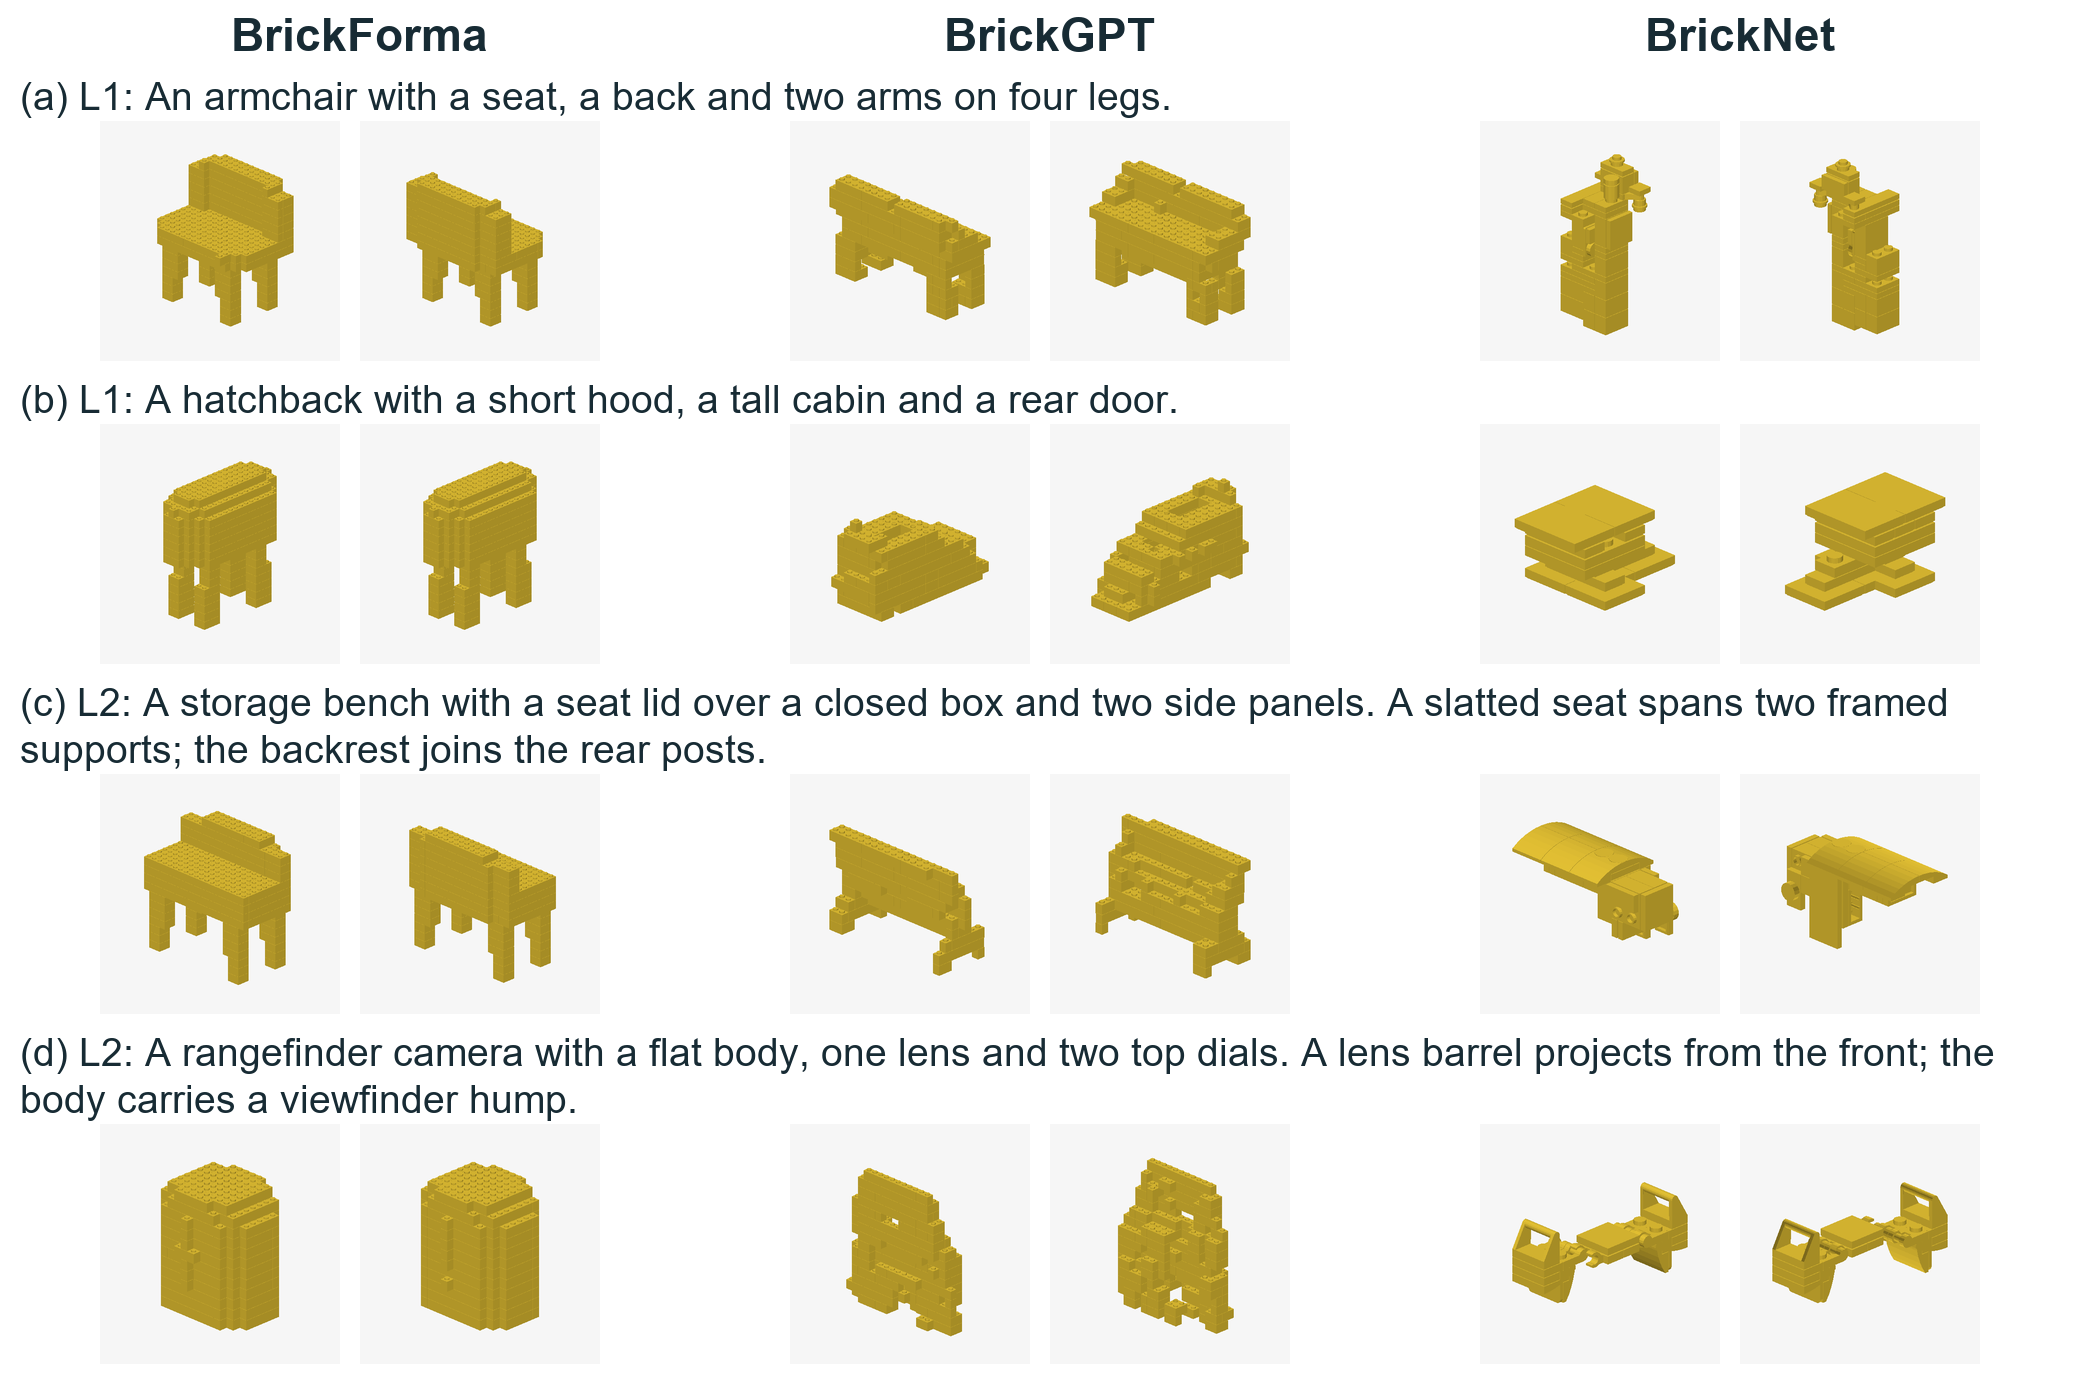
\includegraphics[width=\textwidth]{figures/matched_short_prompts_20261116.png}
\caption{Four matched Group B examples with the same prompts, render settings, and azimuths ($45^\circ$ and $225^\circ$) across systems. The highest VQAScore belongs to BrickForma for the chair and bench, BrickGPT for the hatchback, and BrickNet for the camera.}
\label{fig:gallery}
\end{figure*}


\section{From Text to a Connected Assembly}
\label{sec:model}
\subsection{Learning a Placement Sequence}
\label{sec:training}
We fine-tune Qwen3-1.7B with LoRA on English L1--L5 captions and their checked brick layouts. A model-level 9:1 split keeps descriptions of the same shape together. The $48^3$ grid uses 20 oriented footprints (11 brick sizes up to planar rotation). The instruction lists the allowed dimensions, and the target gives one placement per line, such as $2{\times}4\ (x,y,z)$. Dimensions are serialized Y-first, then X. The sequence describes geometry and omits color.

Fine-tuning follows the BrickGPT Qwen3 script~\cite{brickgpt} (Table~\ref{tab:finetune-config}). Unpacked sequences preserve caption boundaries. The run reached 133,860 steps in 25.3 hours on eight GPUs. Validation loss reached 0.0308 at step 79,000, the released checkpoint, and 0.0339 at the end of epoch 3. Appendix~\ref{app:training} records the validation checkpoints.
\begin{table}[t]
\centering
\small
\setlength{\tabcolsep}{3pt}
\begin{tabular}{@{}l>{\raggedright\arraybackslash}p{0.58\linewidth}@{}}
\toprule
Item & Value \\
\midrule
Base model & Qwen3-1.7B (bf16) \\
Adaptation & LoRA, $r=16$, $\alpha=32$, dropout $0.05$, all linear layers \\
Optimization & LR $10^{-4}$, cosine, 100 warm-up steps, 3 epochs \\
Batch / max length & effective 8 (8 GPUs $\times$ 1) / 8,192 \\
Hardware & DDP, 8$\times$RTX 4090D (24\,GB) \\
Released checkpoint & step 79,000 (best validation loss) \\
Software & transformers 4.51.3, trl 0.17.0, peft 0.15.2 \\
\bottomrule
\end{tabular}
\caption{Fine-tuning configuration (details in Appendix~\ref{app:training}).}
\label{tab:finetune-config}
\end{table}


\subsection{Reconstructing a Single Stud Component}
Algorithm~\ref{alg:inference-retiling} samples with thinking disabled, temperature $0.7$, top-$p$ $0.9$, and at most 8,192 new tokens. It tries seeds 42, 104, and 2026, keeping the first completed draft that passes the geometry validator or the completed draft with the fewest format, library, bounds, and overlap errors. A valid draft with a single stud component is returned as is.

For other drafts, the pipeline forms the in-bounds voxel union $C$ of supported placements, counting overlaps once. Mixed-integer linear programming (MILP) seeks an exact cover of $C$ with one stud-connected component at 12, 60, and 180 seconds. An accepted solution passes an independent audit of placement validity, coverage, and connectivity. If the budget is exhausted, the pipeline can retain the draft and queue a new seed. Recovery runs can sample additional seeds or extend the budget to 600 seconds. We call the drafts \emph{raw} and the accepted reconstructions \emph{retiled}.
